%==============================================================================
%  Final presentation -- VERSION 1: "Classic arc"
%  Problem -> approach -> monotonicity -> experiments -> conclusion.
%  Follows the structure of the report (../Bericht/main.pdf).
%
%  Compile:  latexmk -pdf v1_classic.tex   (biber runs automatically)
%==============================================================================
\documentclass[aspectratio=169, 11pt]{beamer}
\usepackage{finalstyle}
\subtitle{Final Presentation}

\begin{document}

\begin{frame}[plain]
  \titlepage
\end{frame}

\begin{frame}{Outline}
  \tableofcontents
\end{frame}

%==============================================================================
\section{Problem \& Modeling}
%==============================================================================

\begin{frame}{The problem: \drausp{}}
  {\small\textbf{D}ynamic \textbf{R}equest \textbf{A}cceptance and \textbf{U}nsplittable \textbf{S}cheduling \textbf{P}roblem}
  \medskip

  \begin{columns}[T]
    \column{0.4\textwidth}
      \begin{itemize}
        \item $K$ slots with limited capacity; $T_d$ requests arrive one by one.
        \item Request: reward $r$, demand $q$ over \emph{consecutive} slots.
        \item Decide \textbf{immediately and irrevocably}: reject, or accept and choose the start slot.
        \item No splitting, moving or revoking.
      \end{itemize}
      \textbf{Goal:} maximize the total revenue.
    \column{0.6\textwidth}
      \centering
      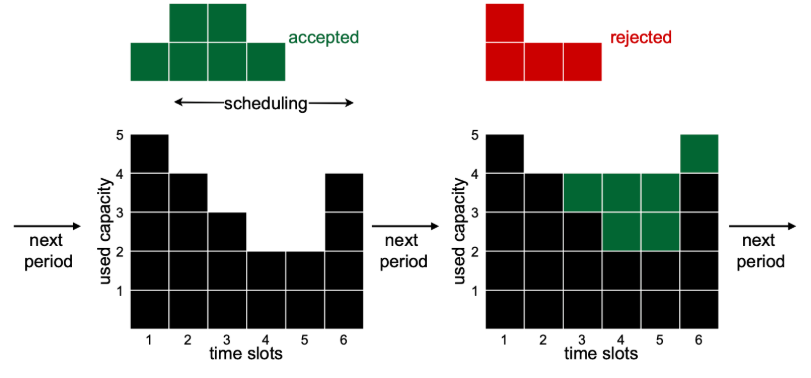
\includegraphics[width=0.95\linewidth]{figures/drausp_example.png}\\
      \hfill{\tiny Figure from~\cite{drausp_lion18}}

      \smallskip
      \begin{alertblock}{The trade-off}
        \small Accepting a low-value request now may use capacity that a more valuable request needs later.
      \end{alertblock}
  \end{columns}
\end{frame}

\begin{frame}{Modeling as an MDP: state space}
  \begingroup\centering
  \begin{tikzpicture}[font=\small,
      cell/.style={draw, minimum width=9.6mm, minimum height=7mm, inner sep=1pt}]
    \foreach \i/\lab/\col in {0/{$t$}/gray!15,
        1/{$\Chat_1$}/blue!10, 2/{$\Chat_2$}/blue!10, 3/{$\Chat_3$}/blue!10, 4/{$\Chat_4$}/blue!10, 5/{$\Chat_5$}/blue!10,
        6/{$r$}/tugreen!15,
        7/{$q_1$}/orange!25, 8/{$q_2$}/orange!25, 9/{$q_3$}/orange!25, 10/{$0$}/gray!5, 11/{$0$}/gray!5}{
      \node[cell, fill=\col] (c\i) at (\i*0.96,0) {\lab};}
    \foreach \a/\b/\lab in {0/0/{time step}, 1/5/{remaining capacities}, 6/6/{reward},
        7/9/{demand}, 10/11/{padding}}{
      \draw[decorate, decoration={brace, mirror, amplitude=4pt}]
        ([xshift=1pt, yshift=-2pt]c\a.south west) -- ([xshift=-1pt, yshift=-2pt]c\b.south east)
        node[midway, below=5pt, font=\scriptsize, align=center] {\lab};}
  \end{tikzpicture}\\[2pt]
  {\scriptsize Example: $K=5$ slots and a request of length $\ell=3$, so the state has $2K+2=12$ entries.}\par
  \endgroup
  \medskip

  \begin{block}{Components}
    \centerline{$s = (t,\ \Chat_1,\dots,\Chat_K,\ r,\ q_1,\dots,q_K) \in \mathbb{R}^{2K+2}$}
    \begin{itemize}
      \item $t \in \{1,\dots,T_d\}$: current decision epoch
      \item $\Chat_k \in \{0,\dots,C_k\}$: remaining capacity of slot $k$
      \item $(r, q)$: the request currently up for decision
    \end{itemize}
    $q$ is zero-padded to length $K$, so requests of any length $\ell$ fit the same state.
  \end{block}
\end{frame}

\begin{frame}{Modeling as an MDP: action space}
  \begin{columns}[T]
    \column{0.5\textwidth}
      \begin{block}{Actions $\mathcal{A} = \{0, 1, \dots, K\}$}
        \begin{itemize}
          \item $a = 0$: reject the request
          \item $a \geq 1$: accept, the block starts at slot $a$
        \end{itemize}
      \end{block}
      \begin{block}{Action $a \geq 1$ is valid only if}
        \begin{enumerate}
          \item the block fits: $a + \ell - 1 \leq K$
          \item every affected slot has enough capacity:\\
            $\Chat_{a+i-1} \geq q_i$ for $i = 1,\dots,\ell$
        \end{enumerate}
      \end{block}
      The valid actions form $\mathcal{A}_s^{\text{valid}}$.
      This set is never empty, because rejecting is always possible.
    \column{0.5\textwidth}
      \centering
      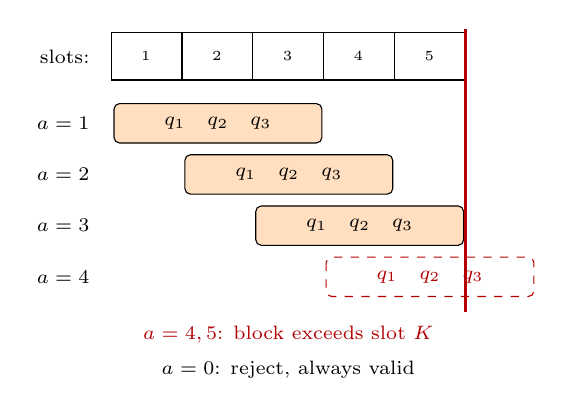
\begin{tikzpicture}[font=\scriptsize,
          slot/.style={draw, minimum width=9mm, minimum height=6mm},
          blk/.style={draw, rounded corners=2pt, fill=orange!25, minimum height=5mm, inner sep=0pt}]
        \foreach \k in {1,...,5}{\node[slot] (s\k) at (\k*0.9,0) {$\Chat_\k$};}
        \node[anchor=east] at (0.3,0) {slots:};
        % candidate placements for a request of length 3
        \foreach \a/\y in {1/-0.85, 2/-1.5, 3/-2.15}{
          \pgfmathsetmacro{\xl}{\a*0.9-0.42}\pgfmathsetmacro{\xr}{(\a+2)*0.9+0.42}
          \node[blk, minimum width={(\xr-\xl)*1cm}, anchor=west] at (\xl,\y) {$q_1 \quad q_2 \quad q_3$};
          \node[anchor=east] at (0.3,\y) {$a=\a$};}
        % a = 4 does not fit
        \draw[dashed, red!70!black, rounded corners=2pt] ({4*0.9-0.42},-2.55) rectangle ({6*0.9+0.42},-3.05);
        \node[text=red!70!black] at ({5*0.9},-2.8) {$q_1 \quad q_2 \quad q_3$};
        \node[anchor=east] at (0.3,-2.8) {$a=4$};
        \draw[red!70!black, thick] ({5*0.9+0.45},0.35) -- ({5*0.9+0.45},-3.25);
        \node[anchor=north, text=red!70!black, align=center] at ({2.7},-3.3) {$a=4,5$: block exceeds slot $K$};
        \node[anchor=north, align=center] at ({2.7},-3.75) {$a=0$: reject, always valid};
      \end{tikzpicture}\\[2pt]
      {\scriptsize Request of length $\ell=3$ with $K=5$ slots.}
  \end{columns}
\end{frame}

\begin{frame}{Modeling as an MDP: transition function and reward}
  \begin{columns}[c]
    \column{0.5\textwidth}
      \centering
      \ProblemGraphic
    \column{0.5\textwidth}
      \begin{block}{Transition $\mathcal{T}(s,a)$, deterministic}
        \begin{itemize}
          \item Accept at slot $a$:\\
            $\Chat_{a+i-1} \leftarrow \Chat_{a+i-1} - q_i$, \ $i=1,\dots,\ell$
          \item Reject: capacities unchanged
          \item Next request $(r_{t+1}, q_{t+1})$ arrives, $t \mapsto t+1$
        \end{itemize}
        Valid actions keep every $\Chat_k \geq 0$.
      \end{block}
      \begin{block}{Reward}
        $\mathcal{R}(s,a)=
          \begin{cases}
            r    & \text{valid accept}\\
            0    & \text{reject}\\
            -100 & \text{invalid, episode ends}
          \end{cases}$
      \end{block}
  \end{columns}
\end{frame}

%==============================================================================
\section{Learning Approach}
%==============================================================================

\begin{frame}{Solving the MDP: from exact optimization to learning}
  \begin{block}{Exact solution}
    Stochastic dynamic programming solves the \drausp{} optimally~\cite{drausp_lion18},
    but becomes intractable as the number of resources and requests grows.
  \end{block}

  \begin{block}{Our approach: reinforcement learning}
    Learn $Q(s,a)$, the expected future revenue of taking action $a$ in state $s$
    and acting optimally afterwards. The policy then acts greedily:
    \[
      \pi(s) = \arg\max_{a} Q(s,a).
    \]
  \end{block}

  \textbf{Goal:} a policy that maximizes the expected total reward over the decision horizon.
\end{frame}

\begin{frame}{Baseline: Standard-DQN with two adaptations}
  \textbf{Deep Q-Network}~\cite{mnih2015}: a neural network outputs one $Q$-value per action;
  using a replay buffer and a target network stabilize training.

  \begin{block}{1. Action masking}
    Despite the penalty, the agent often chose invalid actions.\\
    Invalid actions now get $Q=-\infty$ and are never selected.
  \end{block}

  \begin{block}{2. Reject-biased exploration}
    Random exploration over the valid actions rejects too rarely, which biases the agent towards accepting.\\
    During exploration, we reject with probability $\alpha = 0.75$.
  \end{block}
\end{frame}

%==============================================================================
\section{Monotonicity}
%==============================================================================

\begin{frame}{Which monotonicity is in the problem?}
  Expected relation between a state component and the $Q$-value:

  \medskip
  \begin{center}
  \begin{tabular}{c l l}
    \toprule
    Component & Direction & Intuition \\
    \midrule
    $t$    & \textbf{decreasing} & more time elapsed $\Rightarrow$ fewer future requests can be accepted \\
    $C_k$  & \textbf{increasing} & more remaining capacity $\Rightarrow$ more room for future requests \\
    $r$    & \textbf{increasing} & a higher reward is never valued worse \\
    $q_k$  & \textbf{decreasing} & a higher demand restricts the remaining capacity more \\
    \bottomrule
  \end{tabular}
  \end{center}

  \medskip
  \begin{alertblock}{Core idea}
    A generic network has no guarantee to respect these relations.
    Instead of hoping that it learns them, we \textbf{enforce them in the architecture}.
  \end{alertblock}
\end{frame}

\begin{frame}{Monotonicity test}
  Is enforcing even necessary? First, we need to \textbf{measure} monotonicity.

  \begin{enumerate}
    \item Play episodes with random valid actions and collect the visited states.
    \item For every state $s$, build an \emph{improved} twin $s'$ per component:
      \[
        C' > C, \qquad t' = t-1, \qquad r' = 2r, \qquad q' = q/2,
      \]
      plus a \emph{mixed} twin with all four improvements at once.
    \item Compare the $Q$-values of $s$ and $s'$ for every valid action.
  \end{enumerate}

  \begin{block}{Monotonicity score (one per component)}
    Share of pairs for which the expected relation holds. $1.00$ = perfectly monotone.
  \end{block}
\end{frame}

\begin{frame}{Lattice-DQN: monotone by construction}
  Deep Lattice Network after \textcite{you2017}, used as the $Q$-function:

  \medskip
  \begin{center}
    \LatticePipeline
  \end{center}

  \vspace{-0.3em}
  \begin{columns}[T]
    \column{0.5\textwidth}
      \begin{block}{Why many small lattices?}
        \small One lattice over all $2K{+}2$ state components grows exponentially.
        Many small 3-input lattices keep the same guarantee.
      \end{block}
    \column{0.5\textwidth}
      \begin{block}{Fair comparison}
        \small The Standard-DQN gets the \emph{same number of parameters}
        as the Lattice-DQN on every instance.
      \end{block}
  \end{columns}
\end{frame}

%==============================================================================
\section{Experiments}
%==============================================================================

\begin{frame}{Experimental setup}
  \begin{columns}[T]
    \column{0.5\textwidth}
      \begin{block}{50 benchmark instances~\cite{drausp_lion18}}
        \begin{itemize}
          \item 29 with scheduling (\texttt{SA}, \texttt{SB}, \texttt{SC})
          \item 21 accept/reject only (\texttt{WA}, \texttt{WB}, \texttt{WC})
          \item $K \in \{4, 8, 12\}$ resources
          \item $T_d \in \{5, 10, 20, 50\}$ requests
        \end{itemize}
        Reference: optimal expected value $Z^*$ from exact dynamic programming.
      \end{block}
    \column{0.5\textwidth}
      \begin{block}{Protocol}
        \begin{itemize}
          \item Same training scheme for both agents
          \item $10\,000$ training episodes
          \item Evaluation: frozen weights, no exploration, $10\,000$ episodes
          \item Monotonicity test: $10\,000$ pairs per component
        \end{itemize}
      \end{block}
  \end{columns}
\end{frame}

\begin{frame}{Training on SB05 ($T_d=50$): Standard-DQN}
  \begin{figure}
    \centering
    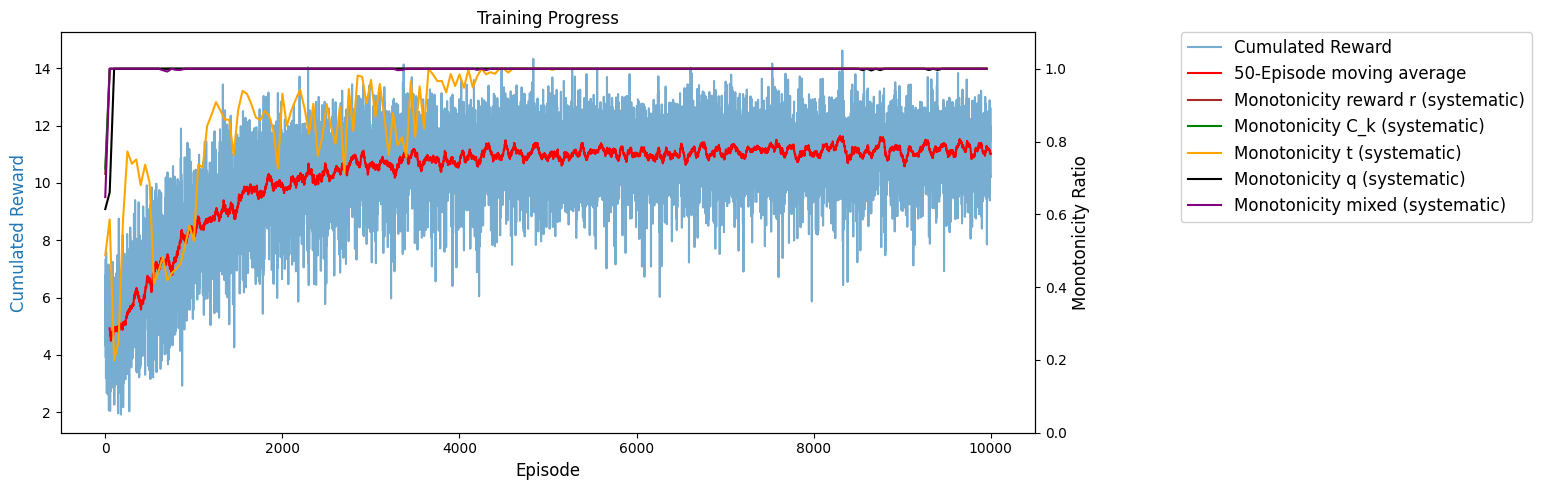
\includegraphics[width=\textwidth,height=0.62\textheight,keepaspectratio]{figures/standard_DQN_mono_SB5_all_new.png}
    \caption{Reward and monotonicity scores over $10\,000$ training episodes.
      $C_k$ and the mixed pairs are learned after a few episodes;
      $t$ first drops, then recovers to $1.00$.}
  \end{figure}
\end{frame}

\begin{frame}{Training on SB05 ($T_d=50$): Lattice-DQN}
  \begin{figure}
    \centering
    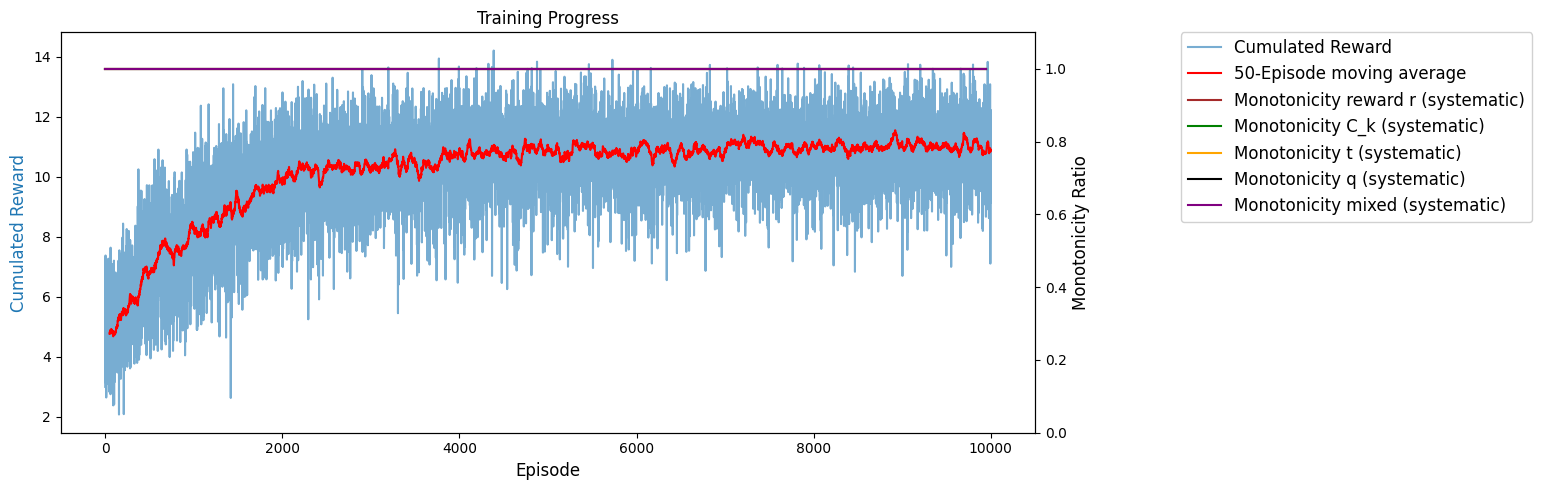
\includegraphics[width=\textwidth,height=0.62\textheight,keepaspectratio]{figures/Deep_Lattice_mono_SB5_all.png}
    \caption{All monotonicity scores are $1.00$ from the first episode (the lines overlap at the top),
      enforced by the architecture.}
  \end{figure}
\end{frame}

\begin{frame}{Reward: how close to the optimum?}
  \begin{columns}[c]
    \column{0.5\textwidth}
      \centering
      \ShareOfOptimumChart{0.9\linewidth}{5.4cm}
      \Source{Mean over all instances per horizon, computed from the report's result tables.}
    \column{0.5\textwidth}
      \small
      \begin{tabular}{l r r r r}
        \toprule
        Instance & $T_d$ & $Z^*$ & Standard & Lattice \\
        \midrule
        SA01 & 10 & 5.08  & \textbf{5.08}  & 5.07 \\
        SA02 & 20 & 8.80  & \textbf{8.58}  & 8.17 \\
        SA03 & 50 & 13.44 & \textbf{13.10} & 12.39 \\
        \addlinespace
        SA04 & 10 & 4.35  & \textbf{4.23}  & 4.16 \\
        SA05 & 20 & 5.97  & \textbf{5.87}  & 5.44 \\
        SA06 & 50 & 7.80  & \textbf{7.62}  & 6.97 \\
        \bottomrule
      \end{tabular}

      \medskip
      \begin{itemize}
        \item \Std: $90$--$100\,\%$ of $Z^*$ on almost all instances.
        \item \Lat: on par on many easier instances, clearly lower at $T_d=50$.
      \end{itemize}
  \end{columns}
\end{frame}

\begin{frame}{Monotonicity: learned vs.\ enforced}
  \centering
  \textbf{\small Standard-DQN: final monotonicity score per component over all 50 instances}\\[2pt]
  \MonotonicityMeanMinChart{0.72\textwidth}{6.3cm}
  \Source{Mean and minimum over all 50 instances, computed from the report's result tables.}
\end{frame}

\begin{frame}{The price of the guarantee}
  \begin{columns}[T]
    \column{0.5\textwidth}
      \centering
      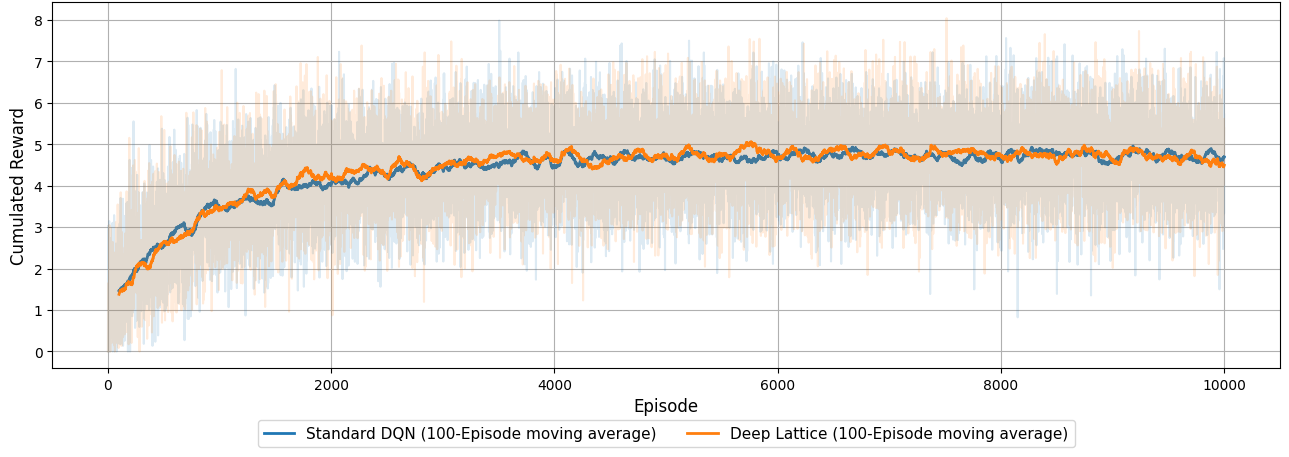
\includegraphics[width=\linewidth]{figures/SB3_vergleich.png}\\
      {\scriptsize SB03, $T_d=10$: similar reward level}
    \column{0.5\textwidth}
      \centering
      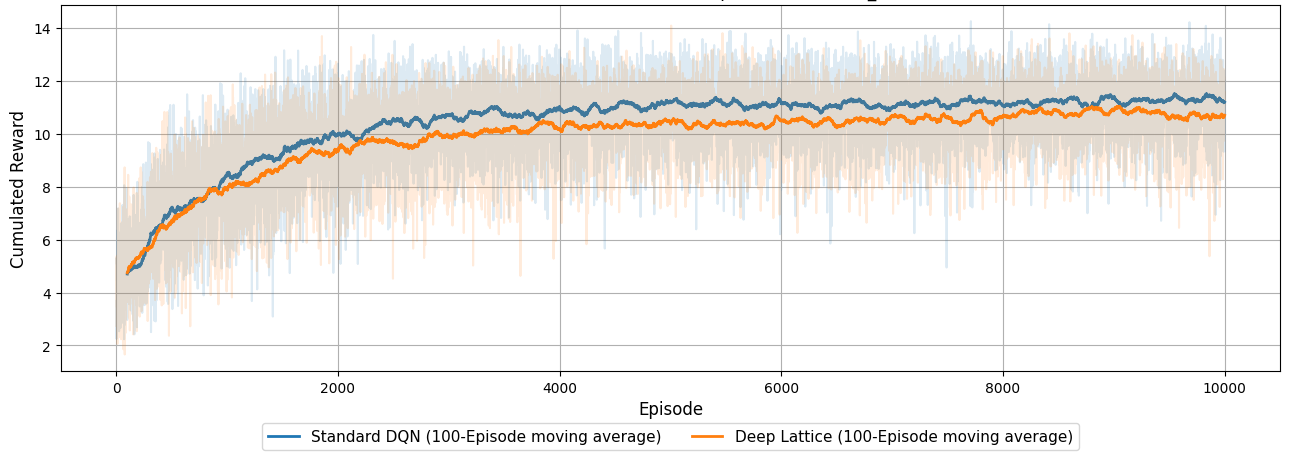
\includegraphics[width=\linewidth]{figures/SB5_vergleich.png}\\
      {\scriptsize SB05, $T_d=50$: Standard-DQN higher}
  \end{columns}

  \medskip
  \begin{itemize}
    \item \textbf{Sample efficiency:} both agents reach a stable level after about $4\,000$ episodes;
      the Lattice-DQN is slightly more unstable at the start.
    \item \textbf{Training time:} the Lattice-DQN trains $5$--$12\times$ slower
      (constraint enforcement after every step, many small lattice evaluations).
    \item \textbf{Tuning:} the Lattice-DQN needs considerably more hyperparameter fine-tuning;
      the Standard-DQN is robust.
  \end{itemize}
\end{frame}

%==============================================================================
\section{Conclusion}
%==============================================================================

\begin{frame}{Conclusion}
  \begin{block}{Results}
    \begin{itemize}
      \item We modeled the \drausp{} as an MDP and built a stable DQN baseline
        with action masking and reject-biased exploration.
      \item The Standard-DQN reaches $90$--$100\,\%$ of the optimum and learns most
        monotonicity relations on its own, but without a guarantee.
      \item The Lattice-DQN satisfies every monotonicity relation exactly.
        Its constrained function class costs reward on long horizons and $5$--$12\times$ training time.
    \end{itemize}
  \end{block}

  \begin{alertblock}{Takeaway}
    Structural monotonicity guarantees reliable, interpretable $Q$-functions,
    at the cost of policy flexibility.
  \end{alertblock}
\end{frame}

\begin{frame}{Limitations \& outlook}
  \begin{columns}[T]
    \column{0.5\textwidth}
      \begin{block}{Limitations}
        \begin{itemize}
          \item One training run per instance and model
          \item Standard deviations reflect only the random requests, not training variability
          \item Several seeds needed to judge significance
          \item No extensive hyperparameter search
        \end{itemize}
      \end{block}
    \column{0.5\textwidth}
      \begin{block}{Outlook}
        \begin{itemize}
          \item Richer lattice architecture: more layers or more lattices per layer
          \item \textbf{Hybrid:} enforce monotonicity only for the relevant features
          \item Early stopping based on out-of-training performance
          \item Does the Standard-DQN still learn monotonicity on larger instances?
        \end{itemize}
      \end{block}
  \end{columns}
\end{frame}

\begin{frame}[allowframebreaks]{References}
  \printbibliography[heading=none]
\end{frame}

\begin{frame}[plain]
  \begin{center}
    {\Huge\textbf{Thank you!}}\\[1em]
    {\large Questions?}
  \end{center}
\end{frame}

\end{document}
